\chapter{Fields}

\textbf{Recall:} $F$ is a field if $F$ is an integral domain (unital) and for all $x \in F \setminus \{0\}$, there exists a multiplicative inverse $x^{-1} \in F \setminus \{0\}$.

In general, there are 3 kinds of fields:
\begin{enumerate}
    \item \textbf{Number field} (a subfield of $\mathbb{C}$) \\ (e.g., $\mathbb{Q}$, $\mathbb{R}$, $\mathbb{Q}(i)$, \dots)
    \item \textbf{Finite field} (a field $F$ with $|F| < \infty$) \\ (e.g., $\mathbb{Z}_p = \mathbb{F}_p$ for $p$ prime. $\mathbb{F}_2[x]/\langle x^3+x+1 \rangle$ has $8=2^3$ elements.)
    \item \textbf{Function fields} \\ (e.g., $\mathbb{C}(x) = \text{Frac}(\mathbb{C}[x]) = \{ f(x)/g(x) \mid f(x), g(x) \in \mathbb{C}[x], g(x) \neq 0 \}$)
\end{enumerate}
We'll only focus on (1) or (2).

\section{Field Extension and Degree}

\textbf{Motivation:} Given a field $F$, construct a "bigger" field $K$ that "contains" $F$.

For example, let $F = \mathbb{F}_2$ and $K = \mathbb{F}_2[x]/\langle x^3+x+1 \rangle$.
Then we have an injective unital ring (or field) homomorphism $i: F \to K$ where $i(0) = 0 + \langle x^3+x+1 \rangle$ and $i(1) = 1 + \langle x^3+x+1 \rangle$. So we say $K$ "contains" $F$.

\begin{definition}
Let $F$ and $K$ be fields. We say $F$ is a \textbf{subfield} of $K$ or $K$ is a \textbf{field extension} of $F$ if there is an injective unital field homomorphism $i: F \to K$.
\end{definition}

In this case, $K$ is a vector space over $F$. There is a scalar multiplication map $\cdot: F \times K \to K$ defined by $\alpha \cdot x = i(\alpha)x$ for $\alpha \in F, x \in K$, that satisfies:
\begin{itemize}
    \item $0 \cdot x = 0$
    \item $1 \cdot x = x$
    \item $\alpha \cdot (x+y) = (\alpha \cdot x) + (\alpha \cdot y)$
    \item \dots
\end{itemize}

The \textbf{degree} of extension is defined as:
\[ [K:F] := \dim_F(K) \quad (\text{as a vector space over } F) \]

\begin{example}
\begin{enumerate}
    \item $F=\mathbb{R}$, $K=\mathbb{C}$, with the inclusion $i: \mathbb{R} \hookrightarrow \mathbb{C}$. \\
    Then $[\mathbb{C}:\mathbb{R}] = 2$, since $\mathbb{C} = \{a+bi \mid a,b \in \mathbb{R}\} = \text{span}_{\mathbb{R}}\{1, i\}$. \\
    Thus, $\dim_{\mathbb{R}}(\mathbb{C}) = 2$ (since $\{1,i\}$ is linearly independent over $\mathbb{R}$).

    \item $F=\mathbb{Q}$, $K=\mathbb{R}$, with the inclusion $i: \mathbb{Q} \hookrightarrow \mathbb{R}$. \\
    To find $[\mathbb{R}:\mathbb{Q}]$, consider that $\mathbb{R} = \text{span}_{\mathbb{Q}}\{1, \sqrt{2}, \sqrt{3}, e, \pi, \dots\}$. \\
    The set of transcendental numbers like $e, \pi$ is infinite and they are linearly independent over $\mathbb{Q}$.
    Thus, $[\mathbb{R}:\mathbb{Q}] = \infty$.
\end{enumerate}
\end{example}

\section{Splitting Extension}
In field theory, we want to understand roots of polynomials $p(x) \in F[x]$. More precisely, we would like to
construct $E:F$ such that $E$ contains some (or all) roots of $F[x]$.
The first step is the following:
\begin{theorem}[Kronecker]
Let $F$ be a field, and $p(x) \in F[x]$ be an irreducible polynomial of degree $m$.
Then $K = F[x]/\langle p(x) \rangle$ is a field extension of $F$ such that $[K:F]=m$.
Moreover, there exists an element $\alpha \in K$ such that:
\begin{itemize}
    \item $K = F[\alpha] := \{a_{n}\alpha^n + \dots + a_1\alpha + a_0 \mid a_i \in F, n \in \mathbb{N} \}$.
    \item $p(\alpha) = 0$ in $K$.
\end{itemize}
\end{theorem}

\begin{proof}
Since $p(x) = b_mx^m + \dots + b_1 x + b_0 \in F[x]$ is irreducible, the ideal $\langle p(x) \rangle$ is a maximal ideal in $F[x]$.
This implies that $K = F[x]/\langle p(x) \rangle$ is a field.

Let's study the dimension, $\dim_F(K)$. Consider the element $\alpha := x + \langle p(x) \rangle \in K$. Then in $K$,
\begin{align*}
p(\alpha) &= b_m \alpha^m + \dots + b_1 \alpha + b_0 \\
&= b_m(x+\langle p(x) \rangle)^m + \dots + b_1(x+\langle p(x) \rangle) + b_0(1+\langle p(x) \rangle) \\
&= (b_m x^m + \dots + b_1 x + b_0) + \langle p(x) \rangle \\
&= p(x) + \langle p(x) \rangle = 0 + \langle p(x) \rangle = 0_K
\end{align*}
So, the second part of the theorem is proved. Moreover, this also implies that 
\[\alpha^m = -\frac{1}{b_m}(b_{m-1}\alpha^{m-1} + \dots + b_0)\] 
i.e. the set $\{1, \alpha, \dots, \alpha^m\}$ is linearly dependent in $K$. More precisely, $\alpha^m$ is a linear combination of $\{1, \alpha, \dots, \alpha^{m-1}\}$.
Similarly, for any $n \ge m$, $\alpha^n$ is also a linear combination of $\{1, \alpha, \dots, \alpha^{m-1}\}$.

\textbf{Claim:} The set $\{1, \alpha, \dots, \alpha^{m-1}\}$ is a basis of $K$ over $F$.

\textbf{Spanning set:} Take any element $k \in K$. By definition, $k = (c_l x^l + \dots + c_1 x + c_0) + \langle p(x) \rangle$ for some $c_i \in F$.
This is equal to $c_l \alpha^l + \dots + c_1 \alpha + c_0$.
Since all powers $\alpha^j$ for $j \ge m$ can be reduced to a linear combination of $\{1, \alpha, \dots, \alpha^{m-1}\}$, any element $k \in K$ can be written as a linear combination of these basis elements.
Thus, $K = \text{Span}_F\{1, \alpha, \dots, \alpha^{m-1}\}$.

\textbf{Linearly independent:} Suppose $d_{m-1}\alpha^{m-1} + \dots + d_1\alpha + d_0 = 0_K$ for some $d_i \in F$, not all zero.
This is equivalent to $(d_{m-1}x^{m-1} + \dots + d_1x + d_0) + \langle p(x) \rangle = 0_K$.
Let $g(x) = d_{m-1}x^{m-1} + \dots + d_0$.
The equation means $g(x) \in \langle p(x) \rangle$.
This implies that $p(x)$ divides $g(x)$, i.e., $g(x) = p(x) \cdot r(x)$ for some $r(x) \in F[x]$.
But this is a contradiction, because $\deg(g(x)) \le m-1$ while $\deg(p(x)) = m$. The degree of a non-zero polynomial $g(x)$ cannot be less than the degree of a non-zero polynomial $p(x)$ that divides it. Thus, $g(x)$ must be the zero polynomial, which means all $d_i$ must be zero.
The set is linearly independent.

Since $\{1, \alpha, \dots, \alpha^{m-1}\}$ is a basis for $K$ over $F$, the dimension is $m$.
Therefore, $[K:F] = m$.
\end{proof}

\begin{example}
Let $F=\mathbb{Q}$, $p(x)=x^3-2 \in \mathbb{Q}[x]$ (irreducible by Eisenstein's criterion).
Then $[K:\mathbb{Q}]=3$ for $K=\mathbb{Q}[x]/\langle x^3-2 \rangle$.
Let $\alpha = x + \langle x^3-2 \rangle$. Then $K = \text{Span}_{\mathbb{Q}}\{1, \alpha, \alpha^2\} = \{a_2\alpha^2+a_1\alpha+a_0 \mid a_i \in \mathbb{Q}\}$.
We know $\alpha^3-2=0$, so $\alpha^3=2$.
$K$ is a field that contains $\mathbb{Q}$ and a cube root of 2. We also know how to do arithmetic in $K$, for instance:
\begin{align*}
(2\alpha^2+\tfrac{3}{4}) \cdot (\alpha-6) &= 2\alpha^3 - 12\alpha^2 + \tfrac{3}{4}\alpha - \tfrac{18}{4} \\
&= 2(2) - 12\alpha^2 + \tfrac{3}{4}\alpha - \tfrac{9}{2} \\
&= 4 - 12\alpha^2 + \tfrac{3}{4}\alpha - \tfrac{9}{2} \\
&= -12\alpha^2 + \tfrac{3}{4}\alpha - \tfrac{1}{2}
\end{align*}
\textbf{Exercise:} What is $\alpha^{-1} \in K$?
\end{example}

In the above example, under the extension $K:\mathbb{Q}$, one can treat the polynomial $p(x) = x^3 - 2 \in \mathbb{Q}[x] \subseteq K[x]$ under the extended field. By Kronecker's theorem, $p(x) \in K[x]$ has a root:
$$p(x) = (x-\alpha)(x^2 + \alpha x + \alpha^2) \in K[x]$$ 
However, $K$ does not contain all the roots of $p(x)$.

\begin{definition}
Let $F$ be a field, and $p(x) \in F[x]$. We say a field extension $E:F$ splits $p(x)$ if
$p(x) = a(x-a_1)\cdots(x-a_n).$
\end{definition}

\begin{proposition}
For any field $F$ and any polynomial $p(x) \in F[x]$, there exists a field extension $E:F$ such that $E$ splits $p(x)$.
\end{proposition}
\begin{proof}
Prove by induction on the degree of $p(x)$ (for any base field $F$). If $p(x) \in F$ is of degree $1$, we are done. By induction hypothesis, assume the theorem holds for all polynomials of degree $< k$ over any field. Consider a polynomial $p(x)$ of degree $k$. Let $f(x)$ be an irreducible factor of $p(x)$.
Then take $K = F[x]/\langle f(x) \rangle$ so that $a := x + \langle f(x) \rangle \in K$ is a root of $f(x)$ and thus of $p(x)$.
So $p(x) = (x-a) g(x)$ in $K[x]$, where $\deg(g(x)) = k-1$.
By the induction hypothesis, there exists an extension $E:K$ such that $g(x)$ splits in $E[x]$, say $g(x) = c(x-a_2)...(x-a_k)$. So we have $p(x) = c(x-a)(x-a_2)...(x-a_k)$ in $E[x]$, and we are done.
\end{proof}

Now we know for any $p(x) \in F[x]$, there is a field extension $E:F$ such that $E$ contains all the roots of $p(x)$. We want to find `the smallest' extension that contains all the roots of $p(x)$.

\begin{definition}
Let $E:F$ be a field extension, and $e_1, \dots, e_n \in E$. Write $F(e_1, \dots, e_n)$ for the smallest field extension of $F$ containing $e_1, \dots, e_n$. In other words,
\[ F(e_1, \dots, e_n) := \bigcap_{K \le E, \ e_1, \dots, e_n \in K} K \]
\end{definition}

\begin{proposition}
$F(e_1, e_2, \dots, e_n) = (F(e_1))(e_2, \dots, e_n) = \dots = ((F(e_1)(e_2))\dots(e_{n-1}))(e_n)$.
\end{proposition}
\begin{proof}
Easy.
\end{proof}

\begin{definition}
Suppose $E:F$ is a field extension such that $E$ splits a polynomial $p(x) \in F[x] \subseteq E[x]$ with roots $a_1, \dots, a_n \in E$. Then a \textbf{splitting field} of $p(x)$ over $F$ is the smallest subfield $F(a_1, \dots, a_n)$ of $E$ containing all the roots $a_i$ of $p(x)$ in E.
\end{definition}

\begin{example}
\
\begin{enumerate}
    \item Let $p(x) = x^2 + 3x + 3 \in \mathbb{Q}[x]$. Then for $E = \mathbb{Q}[x]/\langle p(x) \rangle$, the polynomial $p(x)$ splits automatically into $(x-a)(x-b)$. So $\mathbb{Q}(a,b) = \mathbb{Q}[x]/\langle p(x) \rangle$ is a splitting field.

    On the other hand, $p(x)$ splits in $\mathbb{C}$ and the roots are $-3/2 \pm i\sqrt{3}/2$. So $\mathbb{Q}(i\sqrt{3})$ is also a splitting field of $p(x)$.

    \item Let $p(x) = x^3 - 2 \in \mathbb{Q}[x]$. Then $F = \mathbb{Q}[x]/\langle x^3-2 \rangle$ has a root $\alpha \in E$. We can form $E = F[x]/\langle x^2+\alpha x+\alpha^2 \rangle$. The field $E$ is a splitting field, which we can write as $\mathbb{Q}(a,b,c)$ where $a,b,c$ are the roots.

    On the other hand, working in $\mathbb{C}$, the roots are $2^{1/3}, 2^{1/3}\omega, 2^{1/3}\omega^2$ (where $\omega = e^{i2\pi/3}$). Then $\mathbb{Q}(2^{1/3}, 2^{1/3}\omega, 2^{1/3}\omega^2) = \mathbb{Q}(2^{1/3}, \omega)$ is also a splitting field of $p(x)$.
\end{enumerate}
\end{example}

\begin{theorem} (will prove in MAT5210)
All splitting fields of the same polynomial are isomorphic.
\end{theorem}

\section{Simple Extension}
In the previous section, we begin with a irreducible polynomial $p(x) \in F[x]$,  and extend to $E$ so that $E$ contains some (or all) roots of $p(x)$.
In this section, we change our perspective a little bit – we begin with a field extension $E:F$, and see which elements
in $E$ are roots of a polynomial $p(x) \in F[x]$. Such $E:F$ always exists by the virtue of the previous section.

\begin{definition}
Let $F$ be a field and $L$ be a field extension of $F$ (e.g., $F=\mathbb{Q} \subseteq L=\mathbb{C}$).
An element $\alpha \in L$ is
\begin{itemize}
    \item \textbf{algebraic} if there exists a non-zero polynomial $p(x) \in F[x]$ such that $p(\alpha)=0$ (in $L$).
    \item Otherwise, $\alpha$ is called \textbf{transcendental}.
\end{itemize}
\end{definition}

\begin{example}[Elements over $\mathbb{Q}$]
\
\begin{itemize}
    \item $i = \sqrt{-1}$ is algebraic over $\mathbb{Q}$ (its polynomial is $p(x) = x^2+1$).
    \item $\sqrt[4]{2}, \sqrt{3}$ are algebraic over $\mathbb{Q}$ (their polynomials are $p(x)=x^4-2$ and $x^2-3$, respectively).
    \item $\sqrt{2}+\sqrt{3}$ is algebraic over $\mathbb{Q}$ (HW12).
    \item $e, \pi$ are transcendental over $\mathbb{Q}$ (there is NO polynomial with $\mathbb{Q}$-coefficients having $e$ or $\pi$ as a root).
\end{itemize}
\end{example}

\begin{theorem}
If $\alpha$ is transcendental over $F$, then $F[\alpha] \cong F[x]$ as rings (but not as fields).
\end{theorem}

As for $\beta$ algebraic:
\begin{proposition} \label{prop:minpoly}
Let $\beta \in L$ be algebraic over $F$. Consider the set $I = \{ f(x) \in F[x] \mid f(\beta) = 0 \}$.
Then:
\begin{enumerate}
    \item $I$ is a non-zero ideal in $F[x]$.
    \item $I = \langle p(x) \rangle$ for some unique monic polynomial $p(x) \in F[x]$. (This is because $F[x]$ is a PID).
    \item $p(x)$ is the unique monic polynomial of smallest degree in $I$.
    \item $p(x)$ is irreducible.
\end{enumerate}
This polynomial $p(x)$ is called the \textbf{minimal polynomial} of $\beta$ over $F$.
\end{proposition}

\begin{proof}
(a) Let's show $p(x)$ has the smallest degree. By the division algorithm, suppose on the contrary there exists $g(x) \in I$ with $\deg(g) < \deg(p)$. Since $I=\langle p(x) \rangle$, $g(x)$ must be a multiple of $p(x)$, which is impossible unless $g(x)=0$. Contradiction.

(b) Let's show $p(x)$ is irreducible. Suppose on the contrary that $p(x) = h_1(x)h_2(x)$ with $\deg(h_1) > 0$ and $\deg(h_2) > 0$.
Then $p(\beta) = h_1(\beta)h_2(\beta) = 0$ in the field $L$.
This implies that either $h_1(\beta)=0$ or $h_2(\beta)=0$.
This means either $h_1(x) \in I$ or $h_2(x) \in I$.
But $\deg(h_1) < \deg(p)$ and $\deg(h_2) < \deg(p)$, which contradicts the fact that $p(x)$ is a polynomial of smallest degree in $I$. Thus, $p(x)$ must be irreducible.
\end{proof}

\begin{definition}
Let $F$ be a field, $\beta \in L$ (a field extension of $F$). The polynomial $m_{\beta}(x) := p(x)$ appearing in Proposition \ref{prop:minpoly} above is called the \textbf{minimal polynomial} of $\beta$ over $F$.
\end{definition}

\begin{example}
Minimal polynomials over $\mathbb{Q}$:
\begin{itemize}
    \item For $\beta = i$, the minimal polynomial is $m_{\beta}(x) = x^2+1$.
    \item For $\beta = \sqrt[4]{2}$, the minimal polynomial is $m_{\beta}(x) = x^4-2$.
    \item For $\beta = e^{2\pi i/5}$, the minimal polynomial is $m_{\beta}(x) = x^4+x^3+x^2+x+1$. \\(Since $\beta^5=1$, and $x^5-1 = (x-1)p(x)$).
\end{itemize}
\end{example}

\begin{theorem}
Let $L:F$ be a field extension, and $\beta \in L$ be algebraic. Then the smallest field extension $F(\beta):F$ containing $\beta$ is equal to the polynomial ring $F[\beta]$, which is isomorphic to $F[x]/\langle m_\beta(x) \rangle$.
\end{theorem}

\begin{proof}
Consider the ring homomorphism $\phi: F[x] \to F[\beta]$ defined by evaluation at $\beta$:
\[ \phi(a_n x^n + \dots + a_0) = a_n \beta^n + \dots + a_0 \]
The kernel of this map is precisely the ideal $I = \{ f(x) \in F[x] \mid f(\beta)=0 \}$, which we know is equal to $\langle m_\beta(x) \rangle$.
So the result follows by the First Isomorphism Theorem for rings. Since $\langle m_\beta(x) \rangle$ is a maximal ideal, $F[x]/\langle m_\beta(x) \rangle$ is a field, and therefore $F[\beta]$ is also a field.
\end{proof}

\begin{definition}
The field extension $F(\beta) := F[\beta]$ of $F$ is called the \textbf{simple extension} of $F$ by $\beta$.
\end{definition}

\begin{corollary}
If $\alpha, \beta \in L$ are algebraic over $F$ and are roots of the same irreducible polynomial $p(x) \in F[x]$, then $F(\alpha) \cong F(\beta)$.
\end{corollary}
\begin{proof}
$m_\alpha(x) = m_\beta(x) = p(x)$. So $F(\alpha) \cong F[x]/\langle p(x) \rangle \cong F(\beta)$.
\end{proof}

Let $E:F$ be a field extension, and $\alpha_1, \dots, \alpha_k \in E$ be algebraic over $F$. Then the field extension $F(\alpha_1, \dots, \alpha_k)$ can be constructed inductively as follows:
Define a sequence of fields by $F_0 = F$ and
\[ F_{i+1} := F_i(\alpha_{i+1}) \cong \frac{F_i[x]}{\langle m^{F_i}_{\alpha_{i+1}}(x) \rangle} \quad \text{for } 0 \le i \le k-1. \]
where $m^{F_i}_{\alpha_{i+1}}(x) \in F_i[x]$ is the minimal polynomial of the element $\alpha_{i+1}$ over the field $F_i$. Then $F_k = F(\alpha_1, \dots, \alpha_k)$.

\section{Algebraic Extension}
We have seen that a simple extension $F(\beta):F$ contains an algebraic element $\beta$. What about the other elements in $F(\beta) = \text{Span}_F\{1, \beta, \dots, \beta^{\deg(m_\beta(x))-1}\}$? Are they algebraic? More generally, how about the non-simple extension $F(\beta_1, \dots, \beta_k)$?

\begin{definition}
An extension $E:F$ is called \textbf{algebraic} if every element $\alpha \in E$ is algebraic over $F$.
\end{definition}

\begin{theorem}
If $[E:F] < \infty$ (i.e., it is a finite extension), then $E$ is an algebraic extension of $F$.
\end{theorem}
\begin{proof}
Suppose $[E:F]=n$. Then for any $\alpha \in E$, consider the set $\{1, \alpha, \alpha^2, \dots, \alpha^n\}$. This is a set of $n+1$ elements in an $n$-dimensional vector space, so it must be linearly dependent over $F$.
This implies there exist scalars $c_0, \dots, c_n \in F$, not all zero, such that $c_0 \cdot 1 + c_1 \alpha + \dots + c_n \alpha^n = 0$.
Thus, $\alpha$ is a root of the non-zero polynomial $p(x) = c_nx^n + \dots + c_0 \in F[x]$, which means $\alpha$ is algebraic over $F$. Since $\alpha$ was arbitrary, the extension is algebraic.
\end{proof}

\begin{corollary}
Let $E:F$ be a field extension, and $\beta_1, \dots, \beta_k \in E$ are algebraic over $F$. Then the extension $F(\beta_1, \dots, \beta_k):F$ is algebraic.
\end{corollary}
\begin{proof}
For the special case when $k = 1$, one has $[F(\beta):F] = \deg(m_\beta(x))$ which is finite. The proof of the general case is given in Corollary \ref{cor:extextfinite} below.
\end{proof}

\begin{theorem}[Primitive Element Theorem]
Let $F$ be a field with characteristic $\text{char}(F)=0$. Let $a, b \in K$ be algebraic over $F$ in some extension $K:F$. Then there exists an element $c \in F(a,b)$ such that $F(c) = F(a,b)$. (Such an element $c$ is called a primitive element for the extension).
\end{theorem}

\begin{proof}
Let $p(x)$ be the minimal polynomial of $a$ over $F$.
Let $q(x)$ be the minimal polynomial of $b$ over $F$.

Take a field extension $L:K$ such that $p(x)$ and $q(x)$ split completely in $L[x]$.
Suppose $a_1, \dots, a_m \in L$ are the roots of $p(x)$, with $a_1=a$.
Suppose $b_1, \dots, b_n \in L$ are the roots of $q(x)$, with $b_1=b$.

Since $\text{char}(F)=0$, the field $F$ is infinite. This allows us to choose an element $d \in F$ such that
\[ d \neq \frac{a_i - a_j}{b_k - b_l} \]
for all $i, j$ and for all $k \neq l$. In particular, we choose $d \in F$ such that for any $i$ and any $j > 1$:
\[ d \neq \frac{a_i - a}{b - b_j} \]
(Note that the elements on the right-hand side may not be in $F$, but there are only a finite number of such values, so we can always find a $d \in F$ that avoids them).

Consider the element $c := a + db$.
Then, it is clear that $F(c) \subseteq F(a,b)$ since $a,b \in F(a,b)$ and $d \in F \subseteq F(a,b)$.

To show the other inclusion, $F(a,b) \subseteq F(c)$, it is enough to show that $b \in F(c)$, because if $b \in F(c)$, then $a = c - db \in F(c)$ as well.

Consider the polynomials $r(x) = p(c-dx)$ and $q(x)$, both viewed as polynomials in $F(c)[x]$.
We evaluate both polynomials at $b$:
\begin{itemize}
    \item $r(b) = p(c-db) = p(a) = 0$.
    \item $q(b) = 0$.
\end{itemize}
Let $m(x) \in F(c)[x]$ be the minimal polynomial of $b$ over the field $F(c)$.
Since $b$ is a root of both $r(x)$ and $q(x)$ (which are in $F(c)[x]$), it must be that $m(x)$ divides both $r(x)$ and $q(x)$ in $F(c)[x]$.
\[ m(x) \mid r(x) \quad \text{and} \quad m(x) \mid q(x) \]
Now let's study the polynomial $m(x) \in F(c)[x] \subseteq L[x]$.

Since $m(x) \mid q(x)$ and $q(x)$ splits in $L[x]$, the roots of $m(x)$ must be a subset of the roots of $q(x)$, which are $\{b = b_1, b_2, \dots, b_n\}$.

Consider any root $b_j$ of $m(x)$. Since $m(x)$ also divides $r(x)$, this $b_j$ must also be a root of $r(x)$.
So, for such a $b_j$, we must have $r(b_j) = p(c - db_j) = 0$.
This implies that $c - db_j$ must be one of the roots of $p(x)$, say $a_i$.
\[ c - db_j = a_i \]
Substituting $c=a+db$:
\[ a + db - db_j = a_i \]
\[ d(b - b_j) = a_i - a \]
If $j \neq 1$, then $b \neq b_j$. We can write:
\[ d = \frac{a_i - a}{b - b_j} \]
But this contradicts our initial choice of $d$, which was chosen specifically to not be equal to any of these values.
Therefore, the only possibility is that $j=1$, which means $b_j = b_1 = b$, and hence 
$$m(x) = x - b$$
in $F(c)[x]$, i.e. $b \in F(c)$ and the theorem is proved.
\end{proof}

\section{Tower Law}
\begin{theorem}[Tower Law]
Let $F \subseteq K \subseteq L$ be field extensions.
(e.g., $\mathbb{Q} \subseteq \mathbb{Q}(\sqrt{2}) \subseteq \mathbb{Q}(\sqrt{2}, \sqrt{3})$).
Then:
\[ [L:F] = [L:K] [K:F] \]
\end{theorem}

\begin{proof}
Let $\{e_1, \dots, e_n\}$ be a basis of $K$ over $F$. This means $[K:F] = n$.
Let $\{f_1, \dots, f_m\}$ be a basis of $L$ over $K$. This means $[L:K] = m$.

\textbf{Claim:} The set $\mathcal{B} = \{e_i f_j \mid 1 \le i \le n, 1 \le j \le m\}$ is a basis of $L$ over $F$.
If this claim is true, then the dimension of $L$ over $F$ is $n \cdot m$, which proves the theorem. We need to show that $\mathcal{B}$ is a spanning set and is linearly independent over $F$.

\textbf{Spanning set:}
Let $x$ be any element in $L$. Since $\{f_j\}$ is a basis of $L$ over $K$, we can write $x$ as a linear combination:
\[ x = \sum_{j=1}^{m} \mu_j f_j, \quad \text{where each } \mu_j \in K \]
Now, for each coefficient $\mu_j \in K$, we can express it as a linear combination of the basis elements of $K$ over $F$. For each $j$, we have:
\[ \mu_j = \sum_{i=1}^{n} \nu_{ij} e_i, \quad \text{where each } \nu_{ij} \in F \]
Substituting this back into the expression for $x$:
\[ x = \sum_{j=1}^{m} \left( \sum_{i=1}^{n} \nu_{ij} e_i \right) f_j = \sum_{j=1}^{m} \sum_{i=1}^{n} \nu_{ij} (e_i f_j) \]
Since every element $x \in L$ can be written as a linear combination of the elements $\{e_i f_j\}$ with coefficients $\nu_{ij} \in F$, this set spans $L$ over $F$.

\textbf{Linear Independence:}
Suppose we have a linear combination of the elements $\{e_i f_j\}$ that equals zero, with coefficients $\beta_{ij}$ from the field $F$:
\[ \sum_{i=1}^{n} \sum_{j=1}^{m} \beta_{ij} e_i f_j = 0, \quad \text{where } \beta_{ij} \in F \]
We can regroup the terms by factoring out the $f_j$:
\[ \sum_{j=1}^{m} \left( \sum_{i=1}^{n} \beta_{ij} e_i \right) f_j = 0 \]
For each $j$, the inner sum $\sum_{i=1}^{n} \beta_{ij} e_i$ is a linear combination of elements of the basis $\{e_i\}$ with coefficients in $F$. This means the term in the parenthesis is an element of the field $K$.
So, we have a linear combination of the basis elements $\{f_j\}$ with coefficients from $K$ that equals zero.
By the linear independence of the set $\{f_1, \dots, f_m\}$ over $K$, all the coefficients must be zero:
\[ \sum_{i=1}^{n} \beta_{ij} e_i = 0 \quad \text{for all } j = 1, \dots, m \]
Now, for each $j$, we have a linear combination of the basis elements $\{e_i\}$ over $F$ that equals zero.
By the linear independence of the set $\{e_1, \dots, e_n\}$ over $F$, all the coefficients must be zero:
\[ \beta_{ij} = 0 \quad \text{for all } i,j \]
This shows that the set $\{e_i f_j\}$ is linearly independent over $F$, which completes the proof of the Tower Law. 
\end{proof}

\begin{example}
Let $F = \mathbb{F}_2$ (which is the same as $\mathbb{Z}_2$).
Let $L = \mathbb{F}_2[x]/\langle x^3+x+1 \rangle$.
So, $|L| = 2^3 = 8$ and $[L:F] = 3$.

Are there any proper subfields $K$ with $\mathbb{F}_2 \subset K \subset L$?
Suppose such a subfield $K$ exists. Then by the Tower Law, we must have:
\[ [L:\mathbb{F}_2] = [L:K][K:\mathbb{F}_2] \]
Substituting the known value:
\[ 3 = [L:K][K:\mathbb{F}_2] \]
Since 3 is a prime number and the degrees of extensions are integers greater than or equal to 1, the only possibilities are:
\begin{enumerate}
    \item $[L:K]=1$ and $[K:\mathbb{F}_2]=3$. This implies $K=L$.
    \item $[L:K]=3$ and $[K:\mathbb{F}_2]=1$. This implies $K=\mathbb{F}_2$.
\end{enumerate}
Therefore, there are no proper intermediate subfields between $L$ and $\mathbb{F}_2$.
\end{example}




\begin{corollary} \label{cor:extextfinite}
Suppose we have a tower of fields $F \subseteq E \subseteq K$. If $K:E$ is an algebraic extension and $E:F$ is an algebraic extension, then $K:F$ is also an algebraic extension.
\end{corollary}

\begin{proof}
Let $a \in K$. Since $K:E$ is algebraic, $a$ is a root of some polynomial $p(x) = b_n x^n + \dots + b_1 x + b_0 \in E[x]$.

Since $E:F$ is algebraic, each coefficient $b_i \in E$ is algebraic over $F$.
Consider the tower of fields:
\[ F \subseteq F_0 := F(b_0) \subseteq F_1 := F_0(b_1) \subseteq \dots \subseteq F_n := F_{n-1}(b_n) = F(b_0, \dots, b_n). \]
Since each $b_i$ is algebraic over $F$, it is also algebraic over $F_{i-1}$. Therefore, each extension in this tower, $F_i : F_{i-1}$, is a finite extension. By the Tower Law, $[F_n : F]$ is finite.
\[ [F_n:F] = [F_n:F_{n-1}] \dots [F_1:F_0][F_0:F] < \infty. \]
Now, the polynomial $p(x)$ has its coefficients in $F_n$, so $p(x) \in F_n[x]$. Since $a$ is a root of $p(x)$, the extension $F_n(a):F_n$ is finite, with $[F_n(a):F_n] \le \deg(p) = n$.

Consider the degree of the extension $F_n(a)$ over $F$:
\[ [F_n(a):F] = [F_n(a):F_n][F_n:F]. \]
This product is finite.
Since $F(a)$ is a subfield of $F_n(a)$, we have $[F(a):F] \le [F_n(a):F] < \infty$.
Because $F(a):F$ is a finite extension, it must be an algebraic extension. This implies that the element $a$ is algebraic over $F$.
Since $a$ was an arbitrary element of $K$, the extension $K:F$ is algebraic.
\end{proof}

\begin{corollary}
The set of all algebraic elements in an extension $E:F$ forms a subfield of $E$. 
\end{corollary}
\begin{proof}
Let $a, b \in E$ be algebraic over $F$. We need to show that $a+b$, $a-b$, $ab$, and $a/b$ (for $b \neq 0$) are also algebraic over $F$.
Consider the field $F(a,b)$. By the Tower Law,
\[ [F(a,b):F] = [F(a,b):F(a)][F(a):F]. \]
Since $a$ is algebraic over $F$, $[F(a):F]$ is finite.
Since $b$ is algebraic over $F$, it is also algebraic over the larger field $F(a)$. Thus, $[F(a,b):F(a)] = [F(a)(b):F(a)]$ is also finite.
Therefore, $[F(a,b):F]$ is finite.
Since $F(a,b)$ is a finite extension of $F$, it is an algebraic extension.
Any element of $F(a,b)$ is algebraic over $F$. This includes $a+b, a-b, ab,$ and $a/b$.
\end{proof}

As a final application of the Tower Law:
What can we do with a ruler (with no markings) and a compass?
\begin{itemize}
    \item \textbf{Bisect an angle}
\end{itemize}

\begin{center}
\begin{tikzpicture}[rotate=25,scale=.75]
\tkzDefPoints{0/0/C, 2/-3/A, 4/0/B}
\tkzDefLine[bisector,normed](B,A,C) \tkzGetPoint{a}
\tkzDrawLines[add= 0 and .5](A,B A,C)
\tkzShowLine[bisector,gap=4,size=2,color=red](B,A,C)
\tkzDrawLines[add= 0 and 3](A,a)
\end{tikzpicture}

\end{center}

\textbf{Q:} Can we \textbf{tri-sect} any angle??

\begin{itemize}
    \item \textbf{Double a square}
\end{itemize}

\begin{center}
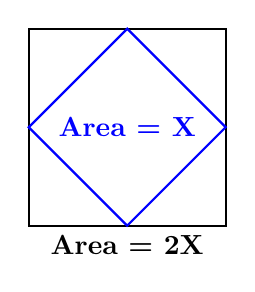
\begin{tikzpicture}[
    % Set a good scale for the drawing
    scale=2.5,
    % Define styles for the elements
    square_style/.style={draw=blue, thick, pattern=north west lines, pattern color=blue!30},
    line_style/.style={draw=black, thick},
    point/.style={circle, fill=black, inner sep=1.5pt}
  ]

  % --- Step 1: Define the vertices of the main bounding box ---
  % This box contains the entire construction.
  \coordinate (A) at (0,1);
  \coordinate (B) at (1,1);
  \coordinate (C) at (1,0);
  \coordinate (D) at (0,0);

  % --- Step 2: Draw the two squares ---
  % They are actually just four triangles, which can be perceived
  % as two different squares.

  % Define the center point
  \coordinate (M) at (0.5, 0.5);

  

  % --- Step 3: Draw the outlines to distinguish the squares ---
  
  % Outline 1: The axis-aligned square (let's call it the 'doubled' one)
  % This square is formed by the outer boundary. Area = 1*1 = 1.
  \draw[line_style] (A) -- (B) -- (C) -- (D) -- cycle;

  % Outline 2: The rotated square (the 'original' one)
  % This square has the center of the edges as its vertices.
  % Its area is half of the larger one.
  \coordinate (p_top) at (0.5, 1);
  \coordinate (p_right) at (1, 0.5);
  \coordinate (p_bottom) at (0.5, 0);
  \coordinate (p_left) at (0, 0.5);

  \draw[line_style, thick, blue] (p_top) -- (p_right) -- (p_bottom) -- (p_left) -- cycle;
  
  \node at (0.5, 0.5) [font=\bf, text=blue] {Area = X};
  \node at (0.5, -0.1) [font=\bf] {Area = 2X};

\end{tikzpicture}
\end{center}

\textbf{Q:} Can you \textbf{double a cube}?